\chapter{Buying the Playbook}

This chapter follows a School of Hard Knocks interview with TJ, a business owner who describes going from food stamps and government cheese to owning multiple companies and reporting roughly nine figures of annual company revenue. The interview is not a blackboard lecture, but it does contain a compact arithmetic of wealth: capped labor income, cash-flowing businesses, debt service, and the surplus that can remain when an acquisition is financed carefully. We will keep the spectacle in its place. The mansion and cars motivate the question; the mechanism is ownership.

\section{The Hook: Revenue, Mansion, and the Problem of Interpretation}

The interview begins with a familiar visual argument: mansion, cars, scale, and a number. TJ is asked for the most money made in a single year across his companies. His answer is approximate but concrete:
\begin{equation}
R_{\mathrm{annual}} \approx \$90\mathrm{M}\text{ to }\$100\mathrm{M}.
\end{equation}
When asked how much was for himself, he gives another figure:
\begin{equation}
I_{\mathrm{personal}} \approx \$25\mathrm{M}.
\end{equation}

Those numbers are claims in an interview, not audited statements. But they tell us what the conversation is trying to explain. We are not asking only, ``How large is the house?'' We are asking what kind of economic machine could make such a house plausible.

The early answer is ownership. TJ says his main business was tech services, that he built it and sold it, then built and sold a construction business, and today has a supplement business. He describes himself as having built businesses and says he owns just under ten companies. The first category, then, is not salary. It is a portfolio of operating claims.

\section{No Rich Parents, No Fixed Definition of Success}

The interviewer next removes the simplest explanation. TJ says he did not come from money. His mother was fourteen when she became pregnant with him; he grew up in the South with food stamps and government cheese. The point is not sentiment. It is the contrast between a poor starting balance sheet and a high-ownership ending position.

He also says he did not begin with a precise hundred-million-dollar target. The early motivation was more primitive: he did not like the environment he was in, wanted to get out, worked, tried to be useful, and kept redefining success as he grew.

\subsection{Question \& Answer}

\paragraph{Question.} Did TJ begin with a clear plan to build a hundred-million-dollar company?

\paragraph{Answer.} No. In the transcript, he says he did not know he wanted a hundred-million-dollar company ``per se.'' What he did know was that he wanted to be successful and did not want to return to the environment he came from. The chapter should preserve that order: motivation before mechanism, motion before map.

\section{The First Rule: Time Is a Capped Asset}

The first general financial rule appears when TJ warns against trading dollars for hours. We can write the simple model as
\begin{equation}
I_{\mathrm{labor}} = w h,
\end{equation}
where \(w\) is the hourly rate and \(h\) is the number of hours worked.

This is not a law of nature, but it captures his claim. If income is tied directly to hours, then even a high rate is limited by the finiteness of time. The cap is not merely psychological; it is structural:
\begin{equation}
h \leq h_{\max}
\qquad\Longrightarrow\qquad
I_{\mathrm{labor}} \leq w h_{\max}.
\end{equation}

That is why TJ moves from work to systems. He says one should make money while sleeping, build systems, invest, and create passive income. In the language of these notes, the goal is to move from a one-person flow of hours to an owned system that can operate when the owner is not directly selling time.

\section{Buying the Playbook}

The interviewer asks what first step someone should take if they are trading time for money and want financial freedom. TJ briefly names real estate, but then pivots: if he were starting today, he would buy businesses.

That pivot matters. He is not primarily recommending that a beginner invent a business from nothing. He says many people want to build from scratch, but today one can ``go get the playbook.'' In other words, an existing business contains evidence: customers, operations, revenue, employees or processes, and visible cash flow.

\subsection{Question \& Answer}

\paragraph{Question.} Why buy instead of build?

\paragraph{Answer.} TJ's answer is that an operating business already has a working playbook. The buyer can see that it works. The opportunity appears because many owners want to leave: their children do not want the business, there may be no succession plan, or the owner needs cash because of divorce, sickness, fatigue, or age. Buying is presented as a way to acquire proof and process at the same time.

\begin{figure}
\centering
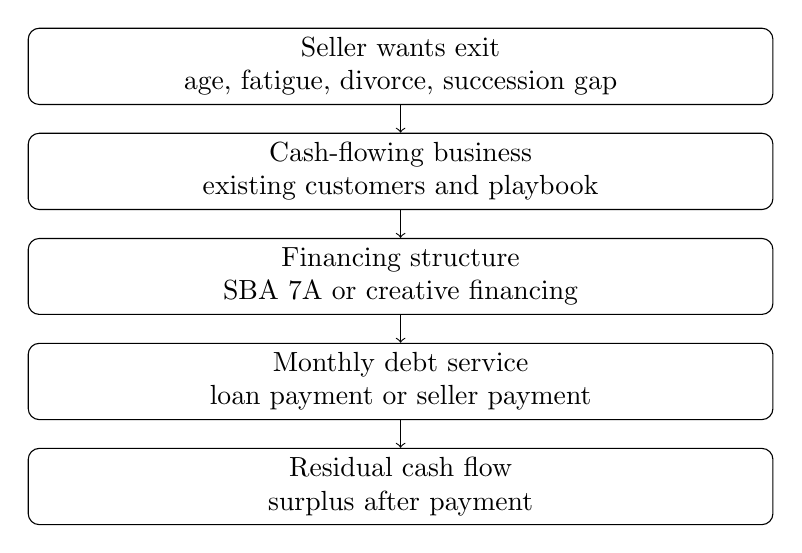
\begin{tikzpicture}[scale=0.92]
\node[draw, rounded corners, align=center, minimum width=0.78\linewidth, minimum height=0.8cm] (seller) at (0,0) {Seller wants exit\\age, fatigue, divorce, succession gap};
\node[draw, rounded corners, align=center, minimum width=0.78\linewidth, minimum height=0.8cm] (business) at (0,-1.45) {Cash-flowing business\\existing customers and playbook};
\node[draw, rounded corners, align=center, minimum width=0.78\linewidth, minimum height=0.8cm] (finance) at (0,-2.90) {Financing structure\\SBA 7A or creative financing};
\node[draw, rounded corners, align=center, minimum width=0.78\linewidth, minimum height=0.8cm] (service) at (0,-4.35) {Monthly debt service\\loan payment or seller payment};
\node[draw, rounded corners, align=center, minimum width=0.78\linewidth, minimum height=0.8cm] (surplus) at (0,-5.80) {Residual cash flow\\surplus after payment};
\draw[->] (seller) -- (business);
\draw[->] (business) -- (finance);
\draw[->] (finance) -- (service);
\draw[->] (service) -- (surplus);
\end{tikzpicture}
\caption{A transcript-grounded reconstruction of TJ's acquisition logic: the opportunity begins with seller exit pressure and only works if the acquired business can carry the financing.}
\end{figure}

\section{The Acquisition Arithmetic}

The most precise numerical mechanism in the interview comes when TJ distinguishes his idea from a vague private-equity slogan. He calls it leveraged buyouts, but the explanation remains simple: find a business that cash flows at a certain number, finance the purchase, service the loan, and keep the spread if the cash flow is larger than the debt service.

Let
\begin{equation}
C_{\mathrm{monthly}} = \text{monthly business cash flow},
\end{equation}
\begin{equation}
D_{\mathrm{monthly}} = \text{monthly debt service},
\end{equation}
and define the monthly surplus by
\begin{equation}
S_{\mathrm{monthly}} = C_{\mathrm{monthly}} - D_{\mathrm{monthly}}.
\end{equation}

TJ's spoken example is:
\begin{equation}
C_{\mathrm{monthly}} = \$20{,}000,
\qquad
D_{\mathrm{monthly}} \in \{\$7{,}000,\ \$10{,}000\}.
\end{equation}
So the illustrative surplus is
\begin{align}
S_{\mathrm{monthly}}
  &= \$20{,}000 - D_{\mathrm{monthly}},\\
  &\in \{\$13{,}000,\ \$10{,}000\}.
\end{align}
The example he emphasizes is the cleaner one:
\begin{equation}
\$20{,}000 - \$10{,}000 = \$10{,}000.
\end{equation}

\subsection{A Worked Example}

Suppose, using TJ's numbers, that a business produces \(\$20{,}000\) per month in the loose sense of cash flow used in the interview. Suppose the acquisition financing requires \(\$10{,}000\) per month in debt service. Then:
\begin{enumerate}
\item The business generates \(C_{\mathrm{monthly}}=\$20{,}000\).
\item The financing consumes \(D_{\mathrm{monthly}}=\$10{,}000\).
\item The monthly surplus is
\[
S_{\mathrm{monthly}} = C_{\mathrm{monthly}} - D_{\mathrm{monthly}}.
\]
\item Substituting the numbers gives
\[
S_{\mathrm{monthly}} = \$20{,}000 - \$10{,}000 = \$10{,}000.
\]
\end{enumerate}

The arithmetic is easy. The hard part is everything hidden inside the word ``cash flow'': the durability of customers, the accuracy of the books, operating risk, repair costs, management time, legal structure, and whether the loan can actually be obtained and serviced. TJ gives the sketch, not a full underwriting manual.

\subsection{Question \& Answer}

\paragraph{Question.} When does leverage help rather than trap the buyer?

\paragraph{Answer.} In the interview's arithmetic, leverage helps only when the acquired business can pay its financing and still leave a margin:
\begin{equation}
C_{\mathrm{monthly}} > D_{\mathrm{monthly}}.
\end{equation}
If the inequality reverses, the buyer has not bought freedom. The buyer has bought a monthly shortfall. The transcript does not give a complete risk model, so the final notes should keep this as a necessary condition, not a guarantee.

\section{What to Buy, and Where Sellers Come From}

TJ names businesses that, in his view, can cash flow without requiring advanced technical know-how from the buyer: laundromats, pool companies, and vending machine businesses. He describes them as less labor intensive and calls them recession-proof. That last phrase should be treated as an interview claim. The safer note is that he is looking for ordinary local services with recurring demand and understandable operations.

\begin{table}
\centering
\begin{tabular}{lll}
Business type & Why TJ mentions it & Caution \\
Laundromat & Cash flow, simple operations & Still needs maintenance and location quality \\
Pool company & Recurring local service & Labor and route management matter \\
Vending machines & Less know-how intensive & Placement and restocking decide economics \\
\end{tabular}
\caption{Transcript-backed examples of businesses TJ names as acquisition targets.}
\end{table}

The next question is where these businesses come from. TJ names several channels:
\begin{itemize}
\item online business-sale portals,
\item business brokers,
\item cold calls to owners who might sell if approached.
\end{itemize}

He then names the broader supply-side thesis: the ``gray tsunami.'' Many older owners have businesses they need to exit, while their children may not want to take them over. The opportunity is therefore not only financial. It is demographic and relational. A buyer is solving a seller's exit problem.

\section{Broke Money, Belief, Skill, and Attention}

After the acquisition mechanics, the interview returns to TJ's internal operating frame. He says he has been broke before, but distinguishes being broke in money from having a broke mindset. He mentions bankruptcy, but says it has been a long time since he has been broke and that he is not going back.

The claim is not that belief substitutes for mechanism. The transcript's order is subtler: belief shapes action, action shapes relationships, and relationships shape opportunity. TJ makes this explicit when discussing faith:
\begin{equation}
\text{belief} \longrightarrow \text{action} \longrightarrow \text{relationships} \longrightarrow \text{opportunity}.
\end{equation}
This is a reconstructed notation for his spoken sequence, not a formal causal law.

College enters in the same practical register. TJ says college did not make him a millionaire, but it did not hurt him. It helped him get a skill set: computer programming, and then a job as a programmer. Skill is useful, but in this lecture it is not the final engine of wealth. It is an entry point.

\subsection{Question \& Answer}

\paragraph{Question.} What lesson about business does TJ say people do not learn in business school?

\paragraph{Answer.} Marketing. His formulation is simple: people may need you, but they do not know who you are. The entrepreneur's job is to identify those people and make the offer visible. In mechanism form:
\begin{equation}
\text{value without attention} \not\Rightarrow \text{growth}.
\end{equation}
The ``magic sauce'' does not matter commercially if the market never sees it.

\section{Environment and the Expansion of the Possible}

The final movement is spatial. The interview walks through a Beverly Park setting and turns nearby houses, celebrity neighbors, and large car collections into a lesson about exposure. TJ says that when one sees certain things, one cannot unsee them. The claim is not that geography mechanically creates wealth. It is that environment can alter the set of possibilities a person considers normal.

We can write the idea schematically:
\begin{equation}
\text{expanded environment} \longrightarrow
\text{expanded vision} \longrightarrow
\text{expanded action set}.
\end{equation}
Again, this is note-taking notation, not a proof. It preserves the structure of his point: seeing larger examples can loosen inherited limits.

The closing contrast is between preset ladders and problem solving. TJ says wealthy people do not live only inside predetermined structures of jobs and raises. They solve problems and create solutions. In the language of the chapter, they seek uncapped systems:
\begin{equation}
\text{wealth path} \approx
\text{ownership} + \text{cash flow} + \text{attention} + \text{expanded constraints}.
\end{equation}

\section{Summary}

The interview begins with the signs of wealth, but its useful payload is a sequence of mechanisms. First, hourly income is capped by time. Second, ownership can separate income from the owner's direct labor. Third, buying an existing cash-flowing business can mean buying an operating playbook rather than inventing one from zero. Fourth, leverage is useful only when the business can service the financing and still leave surplus. Fifth, opportunity often appears because another person needs an exit.

The later sections add the human operating layer: mindset, faith, skill, marketing, environment, and relationships. These are not replacements for arithmetic. In this lecture they are the conditions that shape whether the arithmetic is ever reached.